\documentclass[12pt,a4paper]{article}
\usepackage[english]{babel}
\usepackage{amsmath}
\usepackage{amsfonts}
\usepackage{amssymb}
\usepackage{blindtext}
\usepackage[left=2.54cm,right=2.54cm,top=2.54cm,bottom=2.54cm]{geometry}
\usepackage{ragged2e} 
\usepackage{setspace}
\usepackage{array}
\usepackage{caption}
\usepackage{subcaption}
\usepackage{longtable}
\usepackage{graphicx}
\usepackage{enumitem}
\usepackage{multirow}
%\usepackage[numbers]{natbib}
\usepackage{lscape} % Optional if table is too wide
%\usepackage{hyperref}
\usepackage{lineno}
\usepackage{float}
\usepackage{indentfirst}

\captionsetup{
	labelfont=bf, 
	textfont=it, 
	labelsep=colon, 
	aboveskip=5pt, 
	belowskip=5pt  
}

\newcolumntype{C}[1]{>{\centering\arraybackslash}m{#1}} 
\newcolumntype{L}[1]{>{\raggedright\arraybackslash}m{#1}}
\newcolumntype{R}[1]{>{\raggedleft\arraybackslash}m{#1}} 
\newcolumntype{J}[1]{>{\arraybackslash}m{#1}}
 
\renewcommand{\baselinestretch}{1.15}

\renewcommand{\theequation}{Eq.~\arabic{equation}}

\setlength{\parindent}{1.3cm}
\setlength{\parskip}{1em} 

\begin{document}
	\linenumbers
	
	\begin{justify}
		\textbf{\Large
			Machine Learning Estimation of undrained shear strength of Bangkok clay [Tentative] 
		}
	\end{justify}
	
	\begin{flushleft}
		\textbf{Viroon Kamchoom \textsuperscript{a}, Ankit Garg \textsuperscript{b}, Sai krishna Akash Ramineni \textsuperscript{c}, Thanu Harnpattanapanich \textsuperscript{d,e}, Phichet Ratanaprasatkul \textsuperscript{f}}
	\end{flushleft}
	
	\begin{flushleft}
		{\small {\textsuperscript{a}Excellent centre for green and sustainable infrastructure, Department of Civil Engineering, School of Engineering, King Mongkut's Institute of Technology Ladkrabang (KMITL), Bangkok, Thailand \\ 
				\textsuperscript{b}University in Shantou, Shantou, China \\ 
				\textsuperscript{c}Undergraduate, Department of Civil Engineering at IIT Indore, Indore city, Madhya Pradesh, Postal code- 453552, India \\
				\textsuperscript{d} Geotech Pillar co., ltd, Bangkok, Thailand \\
				\textsuperscript{e} Thailand Underground and Tunnelling Group, The Engineering Institute of Thailand, Thailand \\
				\textsuperscript{f} Bureau of Engineering and Architectural Design, Royal Irrigation Department (RID), Bangkok, Thailand \\
		}}
	\end{flushleft}
	
	\begin{abstract}
		content...
	\end{abstract}
	
	\hspace{0.4cm} \textbf{Keywords:} 
	
	\section{Introduction}
	
	Undrained shear strength (Su), representing the maximum shear stress soil can sustain under undrained conditions, is critical for assessing the short-term stability of geotechnical structures such as foundations and slopes \cite{doi:10.1680/geot.1984.34.4.449}. Its determination traditionally relies on laboratory tests like unconsolidated undrained triaxial and falling cone methods, which face limitations in replicating in-situ stress conditions and microstructure, particularly in complex deposits like Bangkok clay \cite{doi:10.1680/geot.1984.34.4.449,10.1520/GTJ20170127}. While correlations with standard penetration test (SPT) and cone penetration test (CPT) data offer practical alternatives, these methods require site-specific calibration and exhibit substantial uncertainties, with SPT showing poor reliability in soft clays \cite{10.1520/GTJ20170127,ma15186385,Sepúlveda28052025}. Hydrogeological factors, including pore pressure variations, can alter su ratios by over 10\%, emphasizing the need for precise, context-sensitive analyses \cite{belcavello2024influence}.
	
	Bangkok clay presents one of the most challenging geotechnical materials encountered in modern engineering practice, characterized by complex mineralogical composition and highly variable engineering properties that have long troubled infrastructure development in Thailand and similar marine alluvial environments worldwide \cite{phai2019,Pithan_Pairojn_2020}. Recent advances in machine learning technologies have emerged as promising solutions for accurately predicting the undrained shear strength of this problematic soil, offering significant improvements over traditional empirical methods and laboratory testing approaches \cite{app121910177,Demir_Sahin_2024,doi:10.1177/03611981241278354}. Contemporary research demonstrates that sophisticated machine learning models, including hybrid stacking algorithms, random forest, support vector regression, and ensemble methods, can achieve prediction accuracies ranging from 51\% to over 87\% when properly calibrated with comprehensive geotechnical datasets \cite{Demir_Sahin_2024,doi:10.1177/03611981241278354,su12062218}. The integration of advanced data preprocessing techniques, Bayesian optimization algorithms, and multi-algorithm approaches has shown particular promise in addressing the inherent variability and complex behavior of Bangkok clay, while providing more efficient and cost-effective alternatives to extensive field investigation programs \cite{Demir_Sahin_2024,doi:10.1177/03611981241278354,app13095418}.
	
	The clay formation extends to depths of up to 80 meters beneath Bangkok city, with distinct stratifications: a soft, meta-stable layer (4–11 m depth), a stiff clay layer (12–24 m), and deeper hard clay layers, each exhibiting unique microstructural behaviors influenced by geological processes such as sea-level fluctuations and loading-unloading cycles \cite{Krit_Saowiang_Pham_Huy_Giao_2019}. The predominant clay mineral is high-swelling smectite, differentiating it from low-swelling smectite clays like Ariake, and contributing to its high plasticity (liquid limit: 100–140\%, activity: 1.25–1.90) and significant volume change potential \cite{OHTSUBO200011}.These properties, combined with complex responses to chemical treatments and cation exchange, necessitate specialized soil improvement techniques such as Liquefied Stabilized Soil (LSS), Controlled Low Strength Material (CLSM), and liquefied rubber applications to address infrastructure challenges, particularly in pipeline construction \cite{Prum_Jumnongpol_Eamchotchawalit_Kantiwattanakul_Sooksatra_Jarearnsiri_Passananon_2019}.
	
	The study title \lq\lq Modeling Undrained Shear Strength of Sensitive Alluvial Soft Clay Using Machine Learning Approach\rq\rq\ analyzed 111 geotechnical samples of sensitive alluvial clay from Egypt's Nile Delta, using eight easily measurable soil properties as input features: water content ($W_n$), liquid limit ($LL$), dry unit weight ($\gamma_d$), plasticity index ($PI$), consistency index ($CI$), void ratio ($e$), specific gravity ($G_s$), and pocket penetration shear ($q_p$) \cite{app121910177}. These parameters were selected based on their direct physical relationships with undrained shear strength (USS)—for example, higher $LL$, $PI$ and $\gamma_d$ correlated with increased USS due to greater clay content and particle density, while $W_n$ and $e$ showed inverse relationships \cite{app121910177}. The dataset was normalized to address scale disparities, and feature importance analysis confirmed ($q_p$) as the strongest predictor, aligning with its empirical link to field vane shear test results \cite{app121910177}.
	
	Among five machine learning models tested—linear regression, regression trees, Gaussian process regression, ensemble trees, and support vector regression (SVR)—the fine Gaussian SVR achieved superior accuracy, with a testing-set $R^2$ of 0.96 and RMSE of 1.65 \cite{app121910177}. Hyperparameter optimization via Bayesian methods yielded an optimal kernel scale of 8.69 and box constraint ($C$) of 11.83, enabling the model to capture nonlinear interactions between features without overfitting \cite{app121910177}. The SVR’s performance significantly outperformed traditional empirical correlations (e.g., those based solely on $PI$ or $W_n$), demonstrating its utility in bypassing costly field vane tests and disturbed laboratory sampling for USS estimation \cite{app121910177}.
	
	The research titled \lq\lq Prediction of shear strength of soft soil using machine learning methods \rq\rq\ specifically investigates and compares the predictive performance of four machine learning methods—Particle Swarm Optimization Adaptive Network-based Fuzzy Inference System (PANFIS), Genetic Algorithm Adaptive Network-based Fuzzy Inference System (GANFIS), Support Vector Regression (SVR), and Artificial Neural Networks (ANN)—for estimating the shear strength of soft soils. The study utilizes 188 plastic clay soil samples collected from the Nhat Tan and Cua Dai bridge projects in Vietnam, with input variables including moisture content, clay content, liquid limit, plastic limit, plastic index, and consistency index. The models were trained and validated using these datasets, and their performance was assessed using Root Mean Square Error (RMSE) and correlation coefficient (R) \cite{PHAM2018181}.
	
	The findings reveal that PANFIS achieved the highest prediction accuracy (RMSE = 0.038, R = 0.601), outperforming GANFIS (RMSE = 0.04, R = 0.569), SVR (RMSE = 0.044, R = 0.549), and ANN (RMSE = 0.059, R = 0.49). This comparative analysis demonstrates that PANFIS is a promising technique for predicting the strength of soft soils, providing a more effective and accurate alternative to other machine learning approaches tested in this context \cite{PHAM2018181}.
	
	The study \lq\lq Estimation of the undrained shear strength of sensitive clays using optimized inference intelligence system \rq\rq\  introduces two hybrid machine learning models, ANFIS-CA (adaptive neuro-fuzzy inference system with cultural algorithm) and ANFIS-PSO (adaptive neuro-fuzzy inference system with particle swarm optimization), to predict undrained shear strength using five input parameters: depth, effective vertical stress, natural water content, liquid limit, and plastic limit. Unlike traditional empirical models (e.g., Hansbo 1957, Chandler 1988) that rely on error-prone pre-consolidation pressure measurements \cite{Tran_Ho_Van_Le_Prakash_Pham_2022,20210135}, this approach eliminates the need for pre-consolidation data, addressing sampling disturbance challenges common in sensitive clays.
	
	The models were trained on 216 Finnish sensitive clay samples, with ANFIS-PSO achieving superior accuracy (R = 0.715) compared to ANFIS-CA (R = 0.6) \cite{Tran_Ho_Van_Le_Prakash_Pham_2022}. This performance surpasses empirical correlations (R = 0.67–0.71) \cite{20210135}, demonstrating the viability of machine learning for structured clay prediction. Key innovations include metaheuristic optimization (PSO/CA) to refine ANFIS parameters and a focus on vertical effective stress as the most influential input variable (RF weight: 283.33) \cite{Tran_Ho_Van_Le_Prakash_Pham_2022}.
	
	\section{Material and Methods}
	
	\subsection{Soil sample collection and testing}
	
	Soft Bangkok clay samples were collected from two different areas in the western part of Bangkok, Thailand as shown in Figure-\ref{Sample Site Location}. The soil investigation was carried out in order to obtain the design parameters for the water drainage tunnel under Bang Nam Chued and Likij canals, which are part of a national scheme to improve the drainage system and mitigate the recurring inundation problem in the lower Chao Phraya River Basin. A total of 54 boreholes were used in this study. Boreholes with a diameter of 10 cm were drilled using a power auger to a depth of 2–3 meters, and then percussion wash boring was carried out throughout the borehole depth. The soft clay layer was found to vary within 12–15 m depth. The undisturbed samples were collected according to ASTM D1587 by using a Thin-Walled Shelby Tube with a 7.5-cm diameter and a 75-cm length. The samples were collected in soft to medium clay layers at every 1 m. The tube was pressed into the soil about 0.5 m depth and then twisted to take each soil sample out of the borehole. After that, each tube was waxed on both sides to prevent any moisture loss from the soil and transported to the laboratory.
	
	\begin{figure}[H]
		\centering
		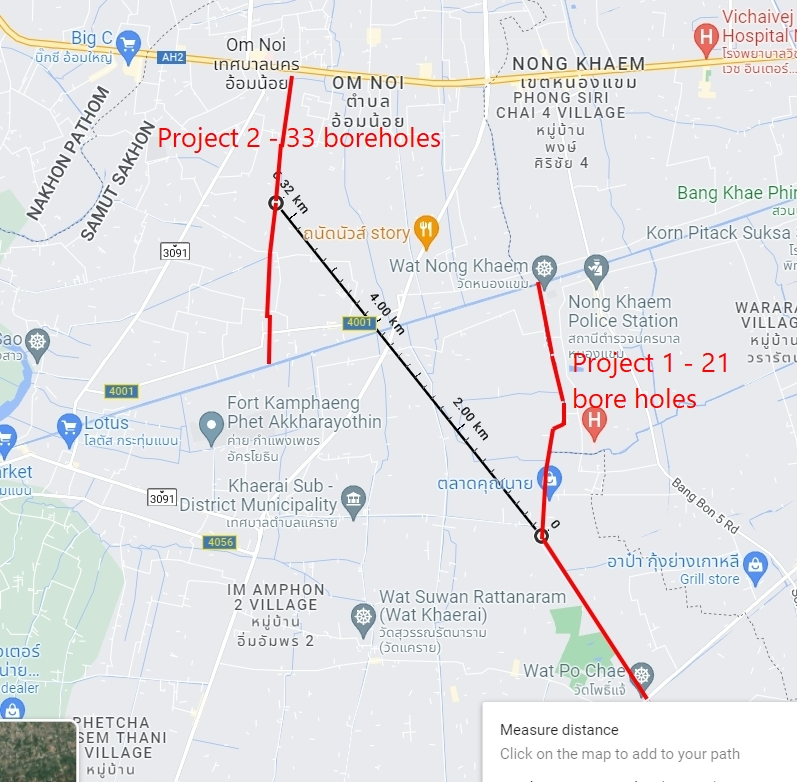
\includegraphics[width=0.75\textwidth]{site location.jpg}
		\caption{Sample Site Location}
		\label{Sample Site Location}
	\end{figure}
	
	The laboratory tests were carried out in accordance with ASTM standards. Bulk unit weight can be calculated from the ratio between the weight of the soil sample and the volume of the soil being measured. The natural water content was calculated based on ASTM D2216, which is the ratio between the weight of soil moisture and the weight of dry soil. The Atterberg limits test according to ASTM D4318 is used to determine the soil index properties that depend on the soil composition, such as mineral compounds in the soil, soil consistency, etc. Grain size distribution was obtained based on ASTM D422. The soil sample was oven-dried at approximately 105 °C for 24 h, after which the dried soil was sieved through a sieve number of 200 (for particles smaller than 75 microns). The hydrometer test according to ASTM D2487 was conducted for soil classification. The limits, such as LL (Liquid limit), PL (Plastic limit), and PI (Plastic Index), together with the grain size distribution, were used to determine the classification of fine-grained soils (i.e., ASTM D2487). The Unconfined Compression Test, referred to as ASTM D21466, was conducted to determine the undrained shear strength of the soil.
	
	\subsection{Machine Learning Framework}
	
	\subsubsection{Dataset Preparation and Preprocessing}
	
	\hspace{1.9cm} Effective preprocessing is foundational in machine learning, as it significantly influences model precision and generalization capabilities \cite{kotsiantis2006data, García_Ramírez-Gallego_Luengo_Benítez_Herrera_2016}. Key operations include data cleaning, feature rescaling, encoding, dimensionality handling, and addressing class distribution issues.
	
	\hspace{1.3cm} In this study, features were standardized using the \textit{Standard Scaler} method, which normalizes input data by subtracting the mean ($\mu$) and dividing by the standard deviation ($\sigma$). The transformation is represented as:
	
	\begin{equation}
		z = \frac{x - \mu}{\sigma}
	\end{equation}
	
	\hspace{1.3cm} To enhance generalization and limit overfitting, normalization was combined with a robust evaluation strategy. An initial 80/20 training-to-testing split was applied. Additionally, five-fold cross-validation was implemented within the training partition to validate model stability and reduce variance \cite{6726842}.
	
	\subsubsection{Regression Models Employed}
	
	\hspace{1.3cm} A variety of regression techniques, ranging from linear to complex ensemble methods, were examined to estimate continuous outcomes \cite{10675076,10934398}. The approach included stages such as preprocessing, model training, hyperparameter optimization, and validation. Model selection was based on complexity, interpretability, and computational efficiency.
	
	\hspace{1.3cm} Table \ref{ML_table} provides a concise summary of the adopted models, their governing equations or loss functions, optimization procedures, and primary considerations.
	
	{\scriptsize \begin{longtable}{C{1.5cm} J{4.5cm} C{4cm} C{4cm}}
			\caption{\label{ML_table} Overview of Regression Techniques and Optimization Approaches} \\
			\hline
			\textbf{Model} & \textbf{Equation / Loss Function} & \textbf{Optimization Strategy} & \textbf{Model Constraints} \\
			\hline
			\endfirsthead
			\hline
			\textbf{Model} & \textbf{Equation / Loss Function} & \textbf{Optimization Strategy} & \textbf{Model Constraints} \\
			\hline
			\endhead
			\hline
			\endfoot
			Linear Regression & 
			\begin{equation}
				Y = \beta_0 + \sum_{i=1}^n \beta_i X_i + \epsilon
			\end{equation}
			OLS objective: 
			\begin{equation}
				\min_\beta \sum_{i=1}^N (y_i - \hat{y}_i)^2
			\end{equation}
			& Closed-form: 
			\begin{equation}
				\beta = (X^TX)^{-1}X^T y
			\end{equation} 
			& 
			\begin{itemize}
				\item $X^TX$ must be invertible
				\item Linearity and homoscedasticity
			\end{itemize} \\
			\hline
			Decision Tree & Predicts by partitioning into leaf nodes & Recursive splitting minimizing node MSE & 
			\begin{itemize}
				\item Control depth and node size
				\item Use pruning to reduce overfitting
			\end{itemize} \\
			\hline
			Random Forest & 
			\begin{equation}
				\hat{y} = \frac{1}{T} \sum_{t=1}^T h_t(x)
			\end{equation} 
			& Bagging of trees on bootstrapped samples & 
			\begin{itemize}
				\item Number of estimators
				\item Feature randomness
			\end{itemize} \\
			\hline
			SVR & 
			\begin{equation}
				\begin{split}
					\min_{w,b} \frac{1}{2}\|w\|^2 + C \sum_{i=1}^{n} (\xi_i + \xi_i^*)
				\end{split}
			\end{equation}
			& Quadratic programming & 
			\begin{itemize}
				\item Kernel function (RBF, poly, linear)
				\item Tuning parameter $C$
			\end{itemize} \\
			\hline
			XGBoost & 
			\begin{equation}
				\hat{y}_i^{(t)} = \hat{y}_i^{(t-1)} + f_t(x_i)
			\end{equation} 
			& Gradient tree boosting & 
			\begin{itemize}
				\item Learning rate
				\item Regularization terms
			\end{itemize} \\
			\hline
			AdaBoost & 
			\begin{equation}
				\hat{y} = \sum_{m=1}^{M} \alpha_m h_m(x)
			\end{equation} 
			& Sequential weighting based on errors & 
			\begin{itemize}
				\item Estimator count
				\item Learning coefficient
			\end{itemize} \\
			\hline
			Gradient Boosting & 
			\begin{equation}
				r_i^{(m)} = y_i - F_{m-1}(x_i)
			\end{equation} 
			& Function space gradient descent & 
			\begin{itemize}
				\item Max tree depth
				\item Estimator count
			\end{itemize} \\
			\hline
			KNN & 
			\begin{equation}
				\hat{y} = \frac{1}{k} \sum_{i \in N_k(x)} y_i
			\end{equation} 
			& Instance-based; no global model & 
			\begin{itemize}
				\item Neighbor count $k$
				\item Distance metric (Euclidean)
			\end{itemize} \\
			\hline
			Gaussian Process & 
			\begin{equation}
				\mu_* = K_*^T K^{-1} y
			\end{equation} 
			& Maximize marginal likelihood & 
			\begin{itemize}
				\item Kernel (e.g., Matérn)
				\item Hyperparameter tuning
			\end{itemize} \\
			\hline
			Neural Networks & 
			\begin{equation}
				MSE = \frac{1}{N} \sum_{i=1}^{N} (y_i - \hat{y}_i)^2
			\end{equation}, 
			\begin{equation}
				MAE = \frac{1}{n} \sum_{i=1}^{n} |y_i - \hat{y}_i|
			\end{equation} 
			& Adam optimizer with backpropagation & 
			\begin{itemize}
				\item Layers: 3; Neurons: 32/layer
				\item ReLU activation
				\item Dropout regularization
				\item Early stopping applied
			\end{itemize} \\
	\end{longtable}}
	
	\hspace{1.3cm} Explanatory symbols: $\beta_0$ and $\beta_i$ are regression intercept and coefficients, respectively. $\epsilon$ denotes residuals, $X^TX$ is the Gram matrix, $y_i$ and $\hat{y}_i$ denote actual and predicted outcomes. In ensemble models, $h_t(x)$ or $f_t(x_i)$ represent weak learners. SVR includes slack variables $\xi_i$ and a margin-control hyperparameter $C$. In KNN, $N_k(x)$ is the set of $k$ nearest neighbors, and in Gaussian Processes, $K$ and $K_*$ denote training and cross-kernel matrices.
	
	\hspace{1.3cm} The study utilized Linear Regression as a foundational benchmark, with Decision Trees and Random Forests selected for their interpretability and non-linear capability. SVR with varying kernels gauged the impact of transformation functions. KNN offered a non-parametric contrast, while ANNs explored high-complexity dependencies. Ensemble approaches like XGBoost, AdaBoost, and GBoost were evaluated for their cumulative correction strategies. Gaussian Process Regression provided probabilistic predictions and uncertainty estimates, supporting robust model comparisons for the soil-biochar interaction task.
	
	\subsubsection{Performance Assessment Criteria}
	
	\hspace{1.3cm} A range of regression performance indicators were applied, including MAE, MSE, RMSE, MAPE, EVS, and both standard and adjusted $R^2$ scores, ensuring a multidimensional evaluation of model accuracy \cite{10958701,Kumar_Khan_Singh_2024}. Table \ref{ele_table} presents the metric formulations.
	
	{\scriptsize \begin{longtable}{C{3cm} J{6cm}}
			\caption{\label{ele_table} Metrics Used to Evaluate Model Performance} \\
			\hline
			\textbf{Metric} & \textbf{Formula} \\
			\hline
			\endfirsthead
			\hline
			\textbf{Metric} & \textbf{Formula} \\
			\hline
			\endhead
			\hline
			\endfoot
			Mean Absolute Error (MAE) & 
			\begin{equation}
				\text{MAE} = \frac{1}{n} \sum_{i=1}^{n} |y_i - \hat{y}_i|
			\end{equation} \\
			Root Mean Squared Error (RMSE) & 
			\begin{equation}
				\text{RMSE} = \sqrt{\frac{1}{n} \sum_{i=1}^{n} (y_i - \hat{y}_i)^2}
			\end{equation} \\
			R-squared ($R^2$) & 
			\begin{equation}
				R^2 = 1 - \frac{\sum (y_i - \hat{y}_i)^2}{\sum (y_i - \bar{y})^2}
			\end{equation} \\
			Adjusted $R^2$ & 
			\begin{equation}
				\bar{R}^2 = 1 - \left( \frac{(1 - R^2)(n - 1)}{n - p - 1} \right)
			\end{equation} \\
	\end{longtable}}
	
	\hspace{1.3cm} Here, $\bar{y}$ is the mean target value, $n$ is the sample size, and $p$ denotes the number of independent variables. These evaluation metrics collectively enabled a nuanced interpretation of model precision, variance capture, and generalizability.
	
	
	
	
	\section{Results and Discussion}
	
	
	
	\section{Conclusion}
	
	\section*{Acknowledgments}
	
	The first author (V. Kamchoom) would like to thank the grant under Climate Change and Climate Variability Research in Monsoon Asia (CMONA) from National Research Council of Thailand (NRCT) and the National Natural Science Foundation of China (NSFC). The second author (A. Garg) thanks the grant XXX provided by XXX. 
	
	\bibliographystyle{unsrt}
	\bibliography{reference.bib}
	\nolinenumbers
\end{document}